%!TEX TS-program = ../make.zsh

\begin{frame}[fragile]{Comparison of parameters from calibration measurements}

  % \begin{columns}
  %   \begin{column}{0.5\textwidth}
  %     \image{angular-acceptance-karle-h2-xaeg2Mee}
  %
  %     \image{angular-acceptance-splicehd-ku3Zie8z}
  %   \end{column}
  %   \begin{column}{0.5\textwidth}
  %     \image{angular-acceptance-dard-eePai1sh}
  %
  %   \end{column}
  % \end{columns}

  \begin{center}
    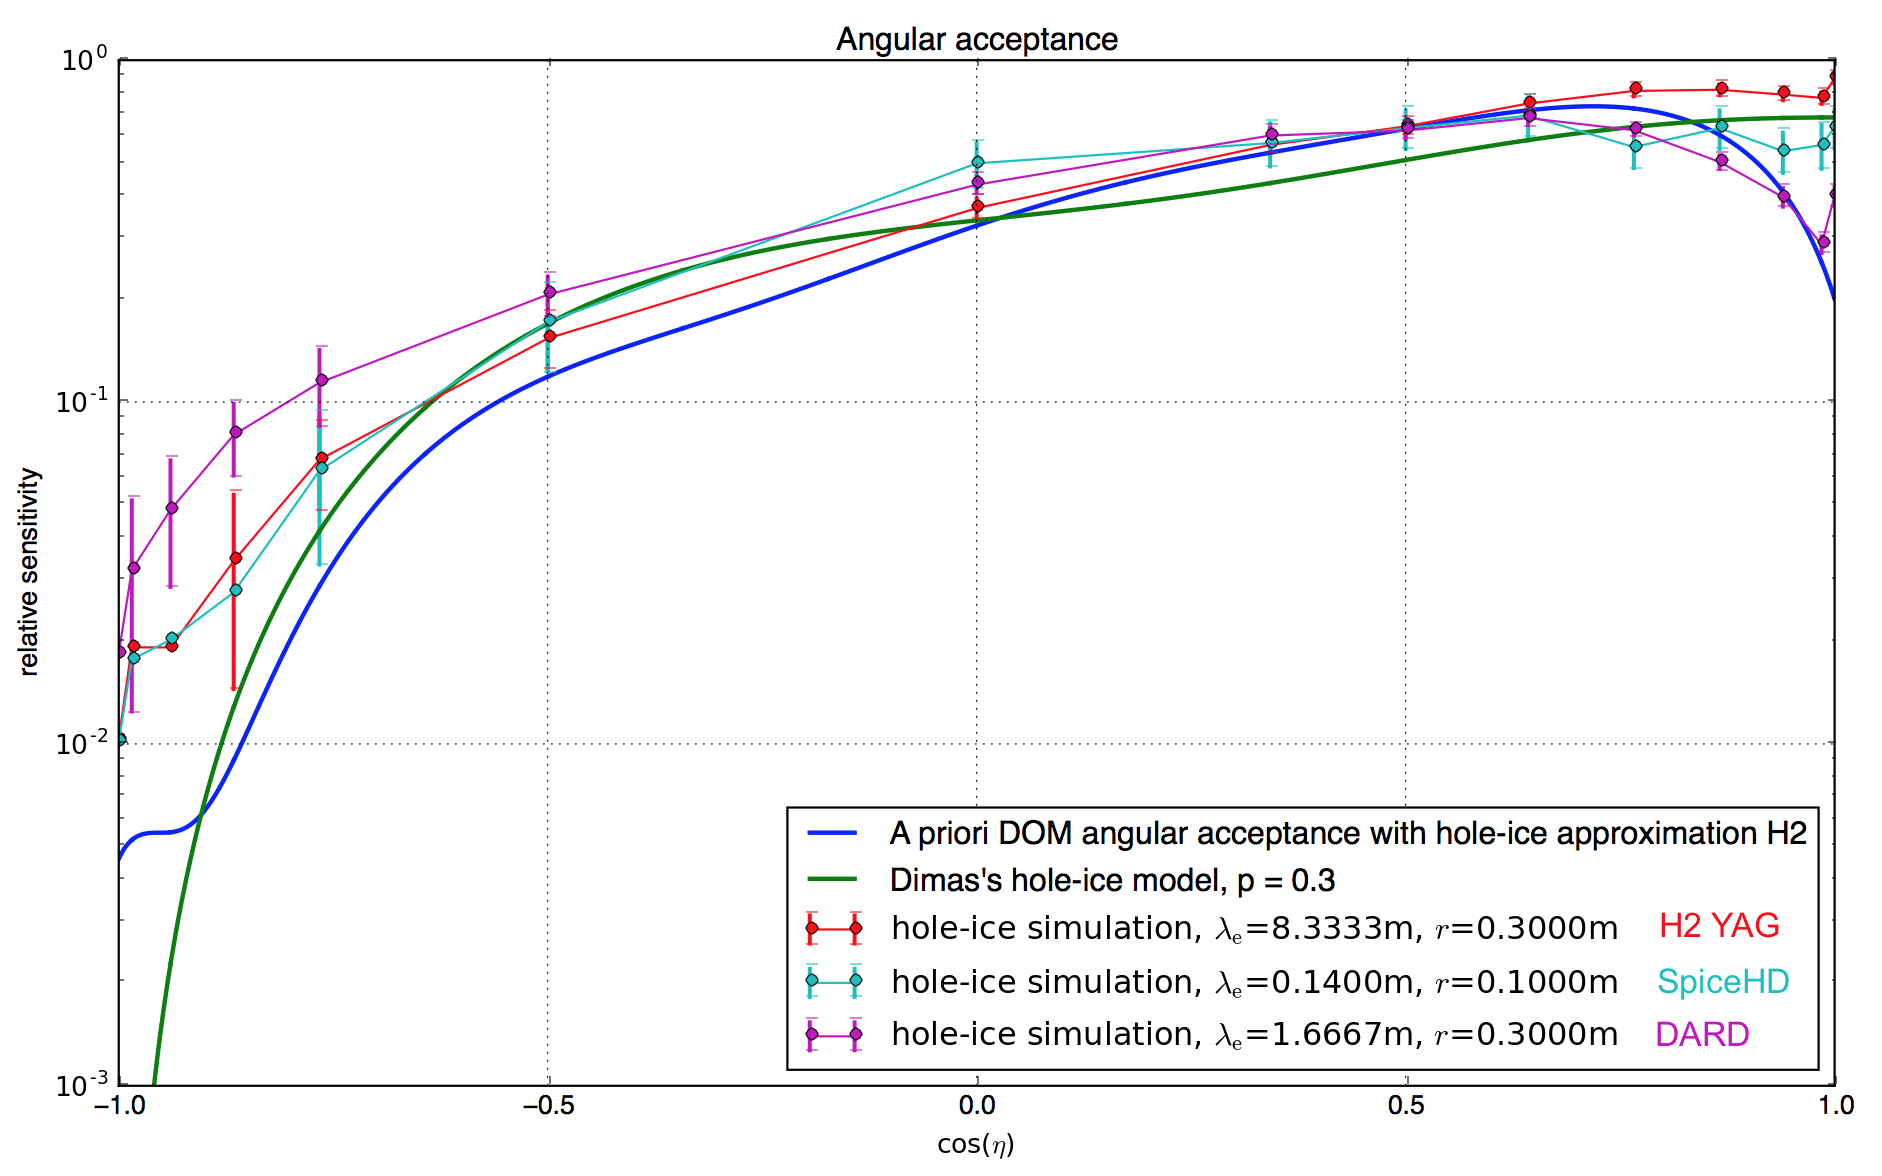
\includegraphics[height=.7\textheight]{img/angular-acceptance-calibration-measurements}
  \end{center}

  \vtiny{%
    \her{Source}:
    \url{https://github.com/fiedl/hole-ice-study/issues/104}
    \her{H2 YAG}: \url{https://github.com/fiedl/hole-ice-study/issues/80}. Karle, Hole Ice Studies with YAG, \url{http://icecube.berkeley.edu/kurt/interstring/hole-ice/yak.html}, 1998.
    \her{SpiceHD}: \url{https://github.com/fiedl/hole-ice-study/issues/87}. Rongen, Status and future of SpiceHD and DARD, Calibration Workshop August 2017.
    \her{DARD}: \url{https://github.com/fiedl/hole-ice-study/issues/105}. Rongen, Measuring the optical properties of IceCube drill holes, 2016. Rongen, DARD Update, Calibration Call 2015-11-06.
  }

\end{frame}